\section{Results}

\subsection{Direct baseline models: LSTM, CNN, and GNN}

The first layer of evidence is the direct three-family comparison that motivated the project before later CNN refinements were merged. Table~\ref{tab:model-comparison} shows the held-out impaired-arm metrics for the original LSTM, CNN, and GNN runs under the shared preprocessing path. No single family dominates every metric. The LSTM is the strongest baseline on exact-match accuracy and macro AUROC, the GNN is best on macro F1 and macro AUPRC, and the legacy CNN is competitive on finger accuracy but otherwise trails the other two branches.

\begin{table}[t]
  \centering
  \small
  \caption{Held-out test performance for the three direct model families. Bold numbers mark the best score in each column within this baseline comparison only.}
  \label{tab:model-comparison}
  \begin{tabular}{lccccc}
\toprule
Model & Subset Acc. & Finger Acc. & Macro F1 & Macro AUROC & Macro AUPRC \\
\midrule
LSTM & \textbf{0.545} & \textbf{0.784} & 0.705 & \textbf{0.858} & 0.754 \\
CNN legacy & 0.442 & 0.694 & 0.676 & 0.767 & 0.764 \\
GNN  & 0.448 & 0.683 & \textbf{0.706} & 0.787 & \textbf{0.776} \\
\bottomrule
\end{tabular}

\end{table}

\begin{figure}[t]
  \centering
  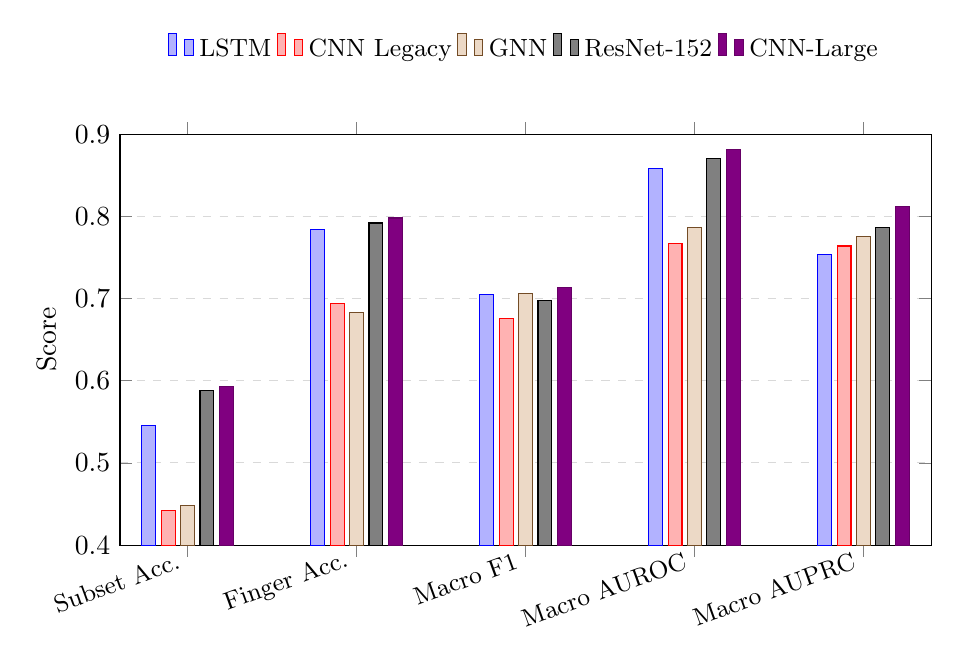
\begin{tikzpicture}
\begin{axis}[
  ybar,
  width=0.98\linewidth,
  height=6.8cm,
  ymin=0.40,
  ymax=0.90,
  ylabel={Score},
  symbolic x coords={Subset Acc.,Finger Acc.,Macro F1,Macro AUROC,Macro AUPRC},
  xtick=data,
  xticklabel style={rotate=20,anchor=east,font=\small},
  ymajorgrids=true,
  grid style={dashed,gray!30},
  legend style={at={(0.5,1.15)},anchor=south,legend columns=-1,draw=none,font=\small},
  bar width=5pt,
]
\addplot coordinates {(Subset Acc.,0.545) (Finger Acc.,0.784) (Macro F1,0.705) (Macro AUROC,0.858) (Macro AUPRC,0.754)};
\addplot coordinates {(Subset Acc.,0.442) (Finger Acc.,0.694) (Macro F1,0.676) (Macro AUROC,0.767) (Macro AUPRC,0.764)};
\addplot coordinates {(Subset Acc.,0.448) (Finger Acc.,0.683) (Macro F1,0.706) (Macro AUROC,0.787) (Macro AUPRC,0.776)};
\addplot coordinates {(Subset Acc.,0.588) (Finger Acc.,0.792) (Macro F1,0.698) (Macro AUROC,0.870) (Macro AUPRC,0.787)};
\addplot coordinates {(Subset Acc.,0.593) (Finger Acc.,0.798) (Macro F1,0.714) (Macro AUROC,0.881) (Macro AUPRC,0.812)};
\legend{LSTM,CNN Legacy,GNN,ResNet-152,CNN-Large}
\end{axis}
\end{tikzpicture}

  \caption{Aggregate-metric comparison across the three direct baselines plus the strongest internal teacher and student references from the newer CNN branch.}
  \label{fig:model-comparison}
\end{figure}

This baseline table is important because it supports the paper's first claim: the project did not begin as a single-model CNN paper. It began as a cross-family study in which recurrent, graph, and convolutional views of the same feature representation each offered different trade-offs. That observation still matters after the newer CNN work is added, because it explains why the repository contains multiple model families and why finger-level analysis remains useful even when one branch improves the aggregate scores.

\subsection{Performance-improvement path: optimized CNN students and ResNet teachers}

The second layer of evidence asks whether the repository's newer CNN branch materially shifts the benchmark frontier. Table~\ref{tab:cnn-sweep} answers yes. Relative to the legacy CNN baseline, the optimized student family improves all major aggregate metrics, and the strongest student, CNN-Large, becomes the best committed model artifact in the repository with 0.593 exact-match accuracy, 0.798 finger accuracy, 0.714 macro F1, 0.881 macro AUROC, and 0.812 macro AUPRC.

\begin{table}[t]
  \centering
  \small
  \caption{Detailed CNN-family evaluation. Student parameter counts and INT8 sizes come from the project CNN README; teacher rows are included as internal high-capacity reference models merged through PR~56. Bold numbers mark the best score in each column across the rows shown.}
  \label{tab:cnn-sweep}
  \resizebox{\linewidth}{!}{\begin{tabular}{llccccccc}
\toprule
Variant & Type & Params & INT8 Size & Subset Acc. & Finger Acc. & Macro F1 & Macro AUROC & Macro AUPRC \\
\midrule
ResNet-50  & Teacher & --    & --      & 0.570 & 0.788 & 0.656 & 0.840 & 0.772 \\
ResNet-101 & Teacher & --    & --      & 0.569 & 0.795 & 0.681 & 0.852 & 0.767 \\
ResNet-152 & Teacher & --    & --      & 0.588 & 0.792 & 0.698 & 0.870 & 0.787 \\
\midrule
Nano        & Student & 54K   & 53 KB   & 0.580 & 0.794 & 0.698 & 0.855 & 0.758 \\
Micro$^\dagger$ & Student & 158K  & 154 KB  & 0.578 & 0.794 & 0.697 & 0.871 & 0.793 \\
Base        & Student & 390K  & 381 KB  & 0.575 & \textbf{0.798} & 0.707 & 0.870 & 0.775 \\
Large       & Student & 803K  & 784 KB  & \textbf{0.593} & \textbf{0.798} & \textbf{0.714} & \textbf{0.881} & \textbf{0.812} \\
XLarge      & Student & 1.62M & 1.58 MB & 0.551 & 0.794 & 0.690 & 0.830 & 0.726 \\
\bottomrule
\end{tabular}
}
\end{table}

Several observations follow from Table~\ref{tab:cnn-sweep}. First, the change from the legacy CNN to the optimized CNN-Large artifact is substantial rather than cosmetic: exact-match accuracy rises from 0.442 to 0.593, macro F1 from 0.676 to 0.714, macro AUROC from 0.767 to 0.881, and macro AUPRC from 0.764 to 0.812. Second, the compact Nano and Micro students remain close to the larger models despite much smaller INT8 footprints, which is the clearest current evidence for the project's edge-oriented design goal. Third, the teacher results provide a meaningful internal reference. Among the committed teacher checkpoints, ResNet-152 is the strongest teacher with 0.588 exact-match accuracy and 0.698 macro F1, yet CNN-Large still slightly exceeds it on exact-match accuracy, macro F1, macro AUROC, and macro AUPRC. This does not prove that distillation is already responsible for the gain, because the repository does not yet commit a comparable distilled-student result set. It does show that the tuned student branch is already competitive with its larger teacher family.

\subsection{Improvement paths for metrics and speed}

Transfer-learning summaries in Table~\ref{tab:transfer-learning} show a deliberately asymmetric result: one path works clearly, one does not. For the CNN branch, healthy-to-impaired staging improves exact-match accuracy from 0.465 to 0.585 and finger accuracy from 0.760 to 0.800 while also improving macro AUROC and macro AUPRC. For the LSTM branch, finetuning improves exact-match and finger accuracy but lowers macro F1, macro AUROC, and macro AUPRC relative to the healthy pretraining summary. The practical conclusion is that healthy-arm pretraining is already a credible improvement path for the CNN family in this repository, but not a universally beneficial recipe across architectures.

\begin{table}[t]
  \centering
  \small
  \caption{Committed healthy-to-impaired transfer-learning summaries. The CNN branch benefits consistently after finetuning; the LSTM branch improves on exact-match and finger accuracy but loses ground on ranking-sensitive metrics.}
  \label{tab:transfer-learning}
  \begin{tabular}{lccccc}
\toprule
Model / Stage & Exact-match & Finger Acc. & Macro F1 & Macro AUROC & Macro AUPRC \\
\midrule
CNN pre. & 0.465 & 0.760 & 0.664 & 0.833 & 0.699 \\
CNN fine. & \textbf{0.585} & \textbf{0.800} & \textbf{0.680} & \textbf{0.863} & \textbf{0.767} \\
LSTM pre. & 0.523 & 0.752 & \textbf{0.679} & \textbf{0.858} & \textbf{0.773} \\
LSTM fine. & \textbf{0.574} & \textbf{0.777} & 0.660 & 0.830 & 0.736 \\
\bottomrule
\end{tabular}

\end{table}

Distillation is best interpreted differently. The repository now contains teacher-ensemble distillation code, explicit multilabel distillation losses, threshold-tuning utilities, and latency-benchmarking scripts, all of which are aligned with the project's goal of improving the speed-quality trade-off for Raspberry Pi-class deployment. However, the current artifact set still lacks a mature distilled-student evaluation bundle and committed on-device timing logs. The distillation story is therefore architectural and procedural rather than empirical at this stage: it is an implemented path for future speed and compression gains, not yet a closed result in the same sense as the direct or transfer tables.

\subsection{Finger-level behavior and external positioning}

Finger-wise scores show that the ranking is not uniform across all outputs. Table~\ref{tab:per-finger-f1} compares the LSTM direct baseline, the GNN direct baseline, and the best optimized CNN student. The GNN remains strongest on the thumb label, the optimized CNN-Large leads on index and little finger, and the LSTM remains slightly strongest on middle and ring finger. This pattern suggests that aggregate CNN gains do not erase all output-specific variation; different inductive biases still matter at the finger level.

\begin{table}[t]
  \centering
  \small
  \caption{Per-finger F1 score by model family. The optimized CNN-Large replaces the legacy direct CNN row for the finger-level comparison. Bold numbers mark the strongest model for each finger.}
  \label{tab:per-finger-f1}
  \begin{tabular}{lccc}
\toprule
Finger & LSTM & GNN & CNN \\
\midrule
Thumb  & 0.716 & \textbf{0.776} & 0.726 \\
Index  & \textbf{0.723} & 0.696 & 0.660 \\
Middle & \textbf{0.712} & 0.689 & 0.675 \\
Ring   & \textbf{0.696} & 0.688 & 0.670 \\
Little & \textbf{0.680} & 0.678 & 0.649 \\
\bottomrule
\end{tabular}

\end{table}

\begin{figure}[t]
  \centering
  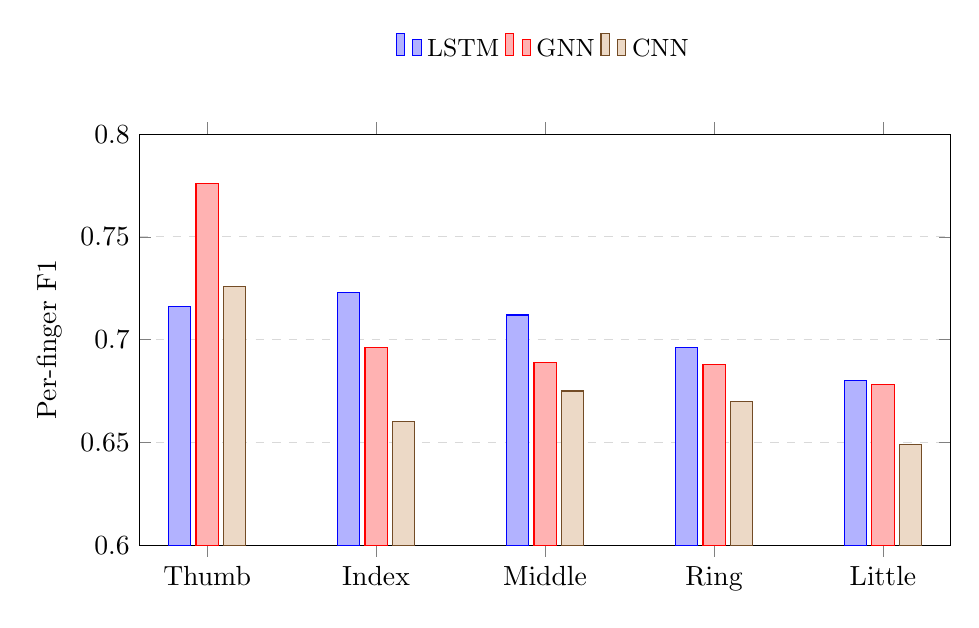
\begin{tikzpicture}
\begin{axis}[
  ybar,
  width=0.98\linewidth,
  height=6.8cm,
  ymin=0.60,
  ymax=0.80,
  ylabel={Per-finger F1},
  symbolic x coords={Thumb,Index,Middle,Ring,Little},
  xtick=data,
  ymajorgrids=true,
  grid style={dashed,gray!30},
  legend style={at={(0.5,1.15)},anchor=south,legend columns=-1,draw=none,font=\small},
  bar width=8pt,
]
\addplot coordinates {(Thumb,0.716) (Index,0.723) (Middle,0.712) (Ring,0.696) (Little,0.680)};
\addplot coordinates {(Thumb,0.776) (Index,0.696) (Middle,0.689) (Ring,0.688) (Little,0.678)};
\addplot coordinates {(Thumb,0.726) (Index,0.660) (Middle,0.675) (Ring,0.670) (Little,0.649)};
\legend{LSTM,GNN,CNN}
\end{axis}
\end{tikzpicture}

  \caption{Per-finger F1 comparison derived from the committed metric files. Aggregate CNN gains coexist with output-specific strengths for the LSTM and GNN baselines.}
  \label{fig:per-finger-f1}
\end{figure}

To show where this project stands relative to the literature, Table~\ref{tab:literature-context} should be read alongside the internal results rather than against them. Prior stroke-decoding papers often report much higher accuracies than our exact-match scores, but they typically solve easier multiclass tasks with fewer gestures, fewer labels, smaller cohorts, or healthy-data pretraining. Our current numbers are stricter in at least three ways: they use a five-finger multilabel formulation, they are derived from impaired-arm \physiomio\ recordings with patient-level splits, and the headline exact-match metric requires all five finger labels to be correct simultaneously. For that reason, the more meaningful external takeaway is not that \repo\ already leads the literature, but that it now occupies a technically credible position: stronger than a simple proof-of-concept, richer than a single-model benchmark, and explicit enough to support future work on transfer, distillation, and embedded deployment.

The results should nevertheless be read with an evidence boundary in mind. The project now includes code for teacher-ensemble distillation, per-finger threshold tuning, and CPU latency measurement, but it does not yet commit a mature result bundle produced by those new utilities, nor does it store on-device Raspberry Pi 5 timings. The current paper can therefore support a stronger research narrative than the previous draft, but not a full claim of embedded deployment readiness.
